\label{testmiljo}
I dette afsnit præsenteres det testmiljø, der sat op til at teste robottens færdigheder.

\section{Formål}
Formålet med et testmiljø er at bedre kunne kontrollere omgivelserne.
Dette giver mindre unøjagtigheder, ift. hvis det skulle testes i et nyt miljø hver gang, og gør det dermed muligt at sammenligne resultater.

\section{Opsætning}\label{testmiljo:opsaetning}
Testmiljøet er opsat vha. papkasser og tape, som man kan se på \cref{testmiljo:perspektiv}.
Størrelsen er $189 \ cm \times 261 \ cm$. 
Denne størrelse er valgt, da dette præcis passer ift. Kinectens billede, som man kan se på \cref{testmiljo:oppefra}.
På \cref{testmiljo:forfra} kan man se hvordan Kinecten er monteret under en loftplade i forhold til gulvet.

\begin{figure}
\centering
\begin{tikzpicture}
\node[anchor=south west,inner sep=0] at (0,0) {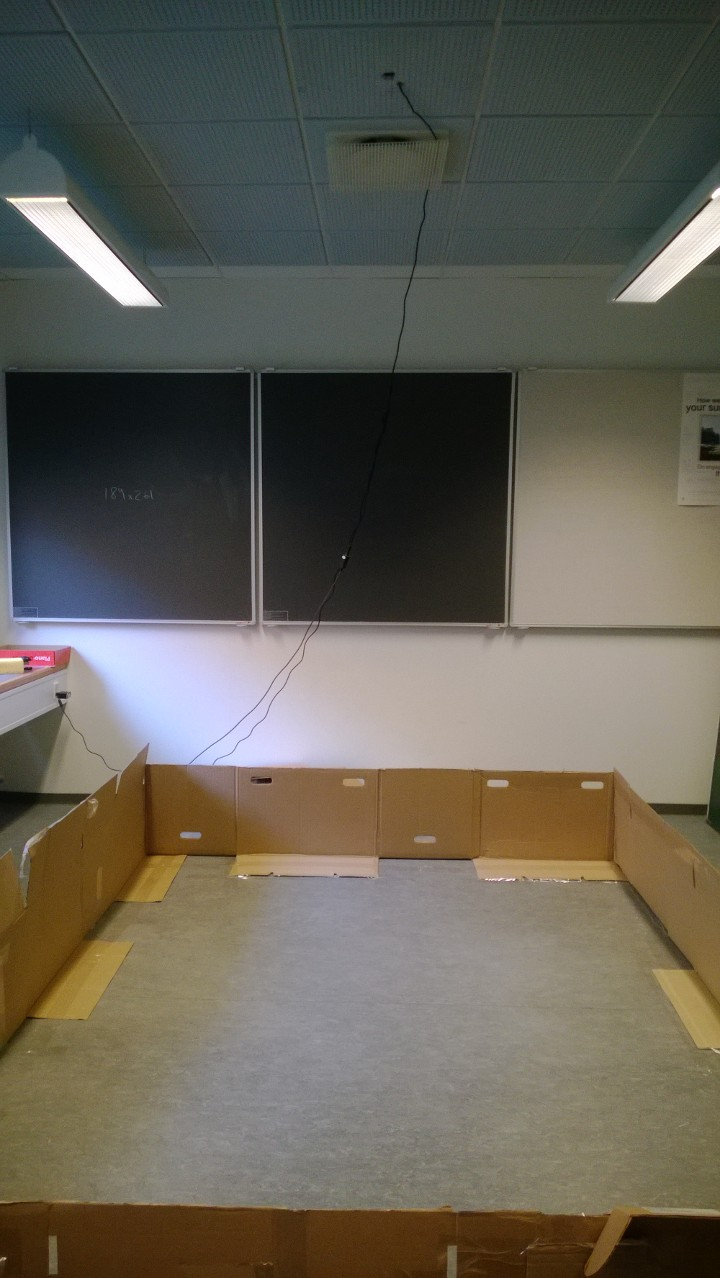
\includegraphics[width=\textwidth/2]{./verden/forfra}};
    \draw [->, red, ultra thick] (5.5,10.5) -- (4.2,11.2);
\end{tikzpicture}
\caption{Testmiljøet set forfra. Bemærk Kinecten monteret i en loftsplade (rød pil) med hul til RGB-kameraet.}
\label{testmiljo:forfra}
\end{figure}

\begin{figure}
\centering
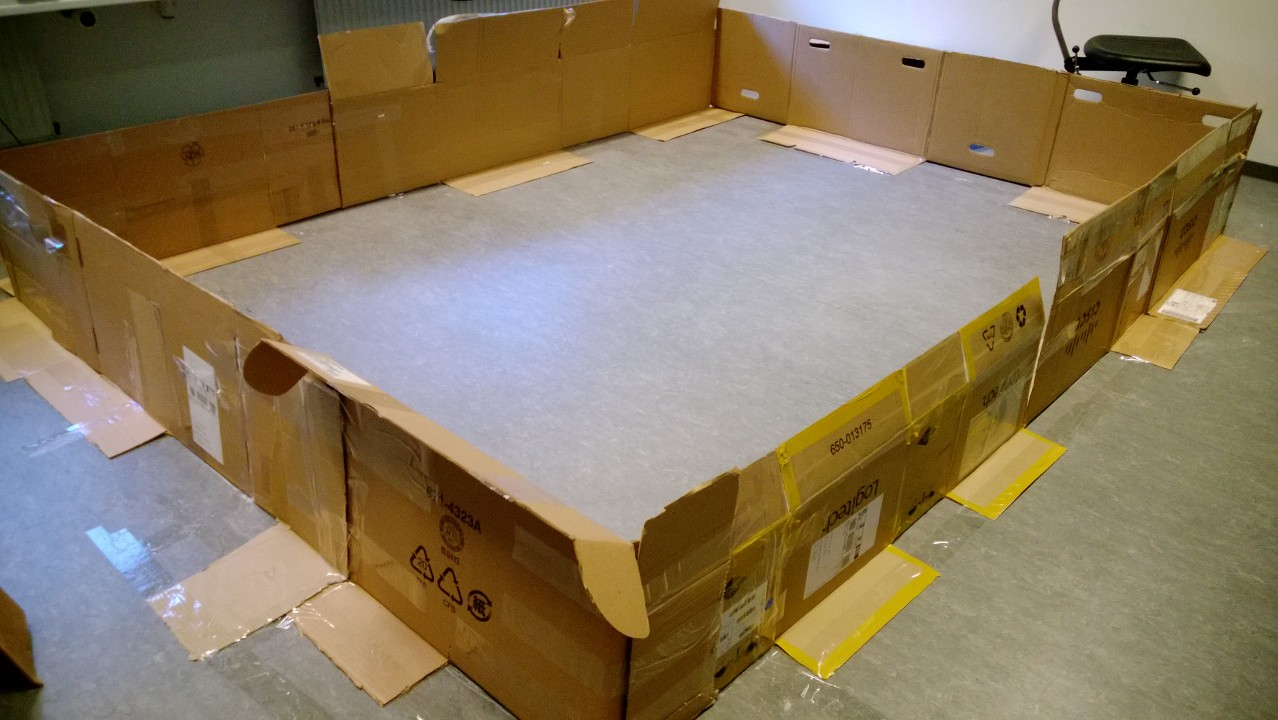
\includegraphics[width=\textwidth]{./verden/perspektiv}
\caption{Testmiljøet set i perspektiv.}
\label{testmiljo:perspektiv}
\end{figure}

\begin{figure}
\centering
\begin{tikzpicture}
\node[anchor=south west,inner sep=0] at (0,0) {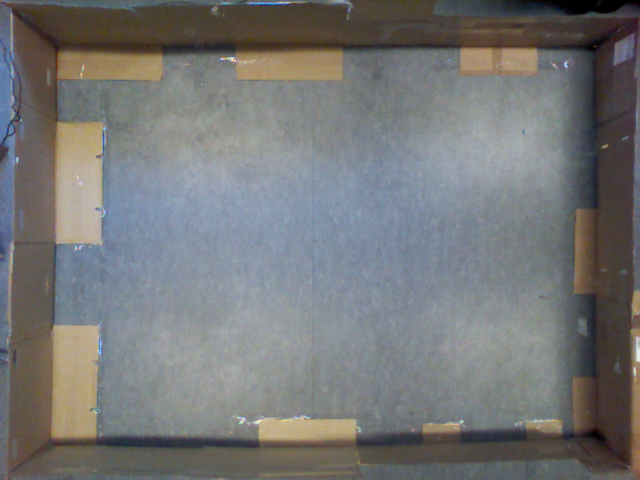
\includegraphics[width=\textwidth]{./verden/oppefra}};
    \draw [<->, red, ultra thick] (1.2,0.9) -- (1.3,9.2);
    \node [red, ultra thick] at (2.5,4.5) {189 cm};
    \draw [<->, red, ultra thick] (1.2,0.9) -- (13,1);
    \node [red, ultra thick] at (7, 1.5) {261 cm};
\end{tikzpicture}
\caption{Testmiljøet set fra Kinecten.}
\label{testmiljo:oppefra}
\end{figure}

\begin{figure}
\centering
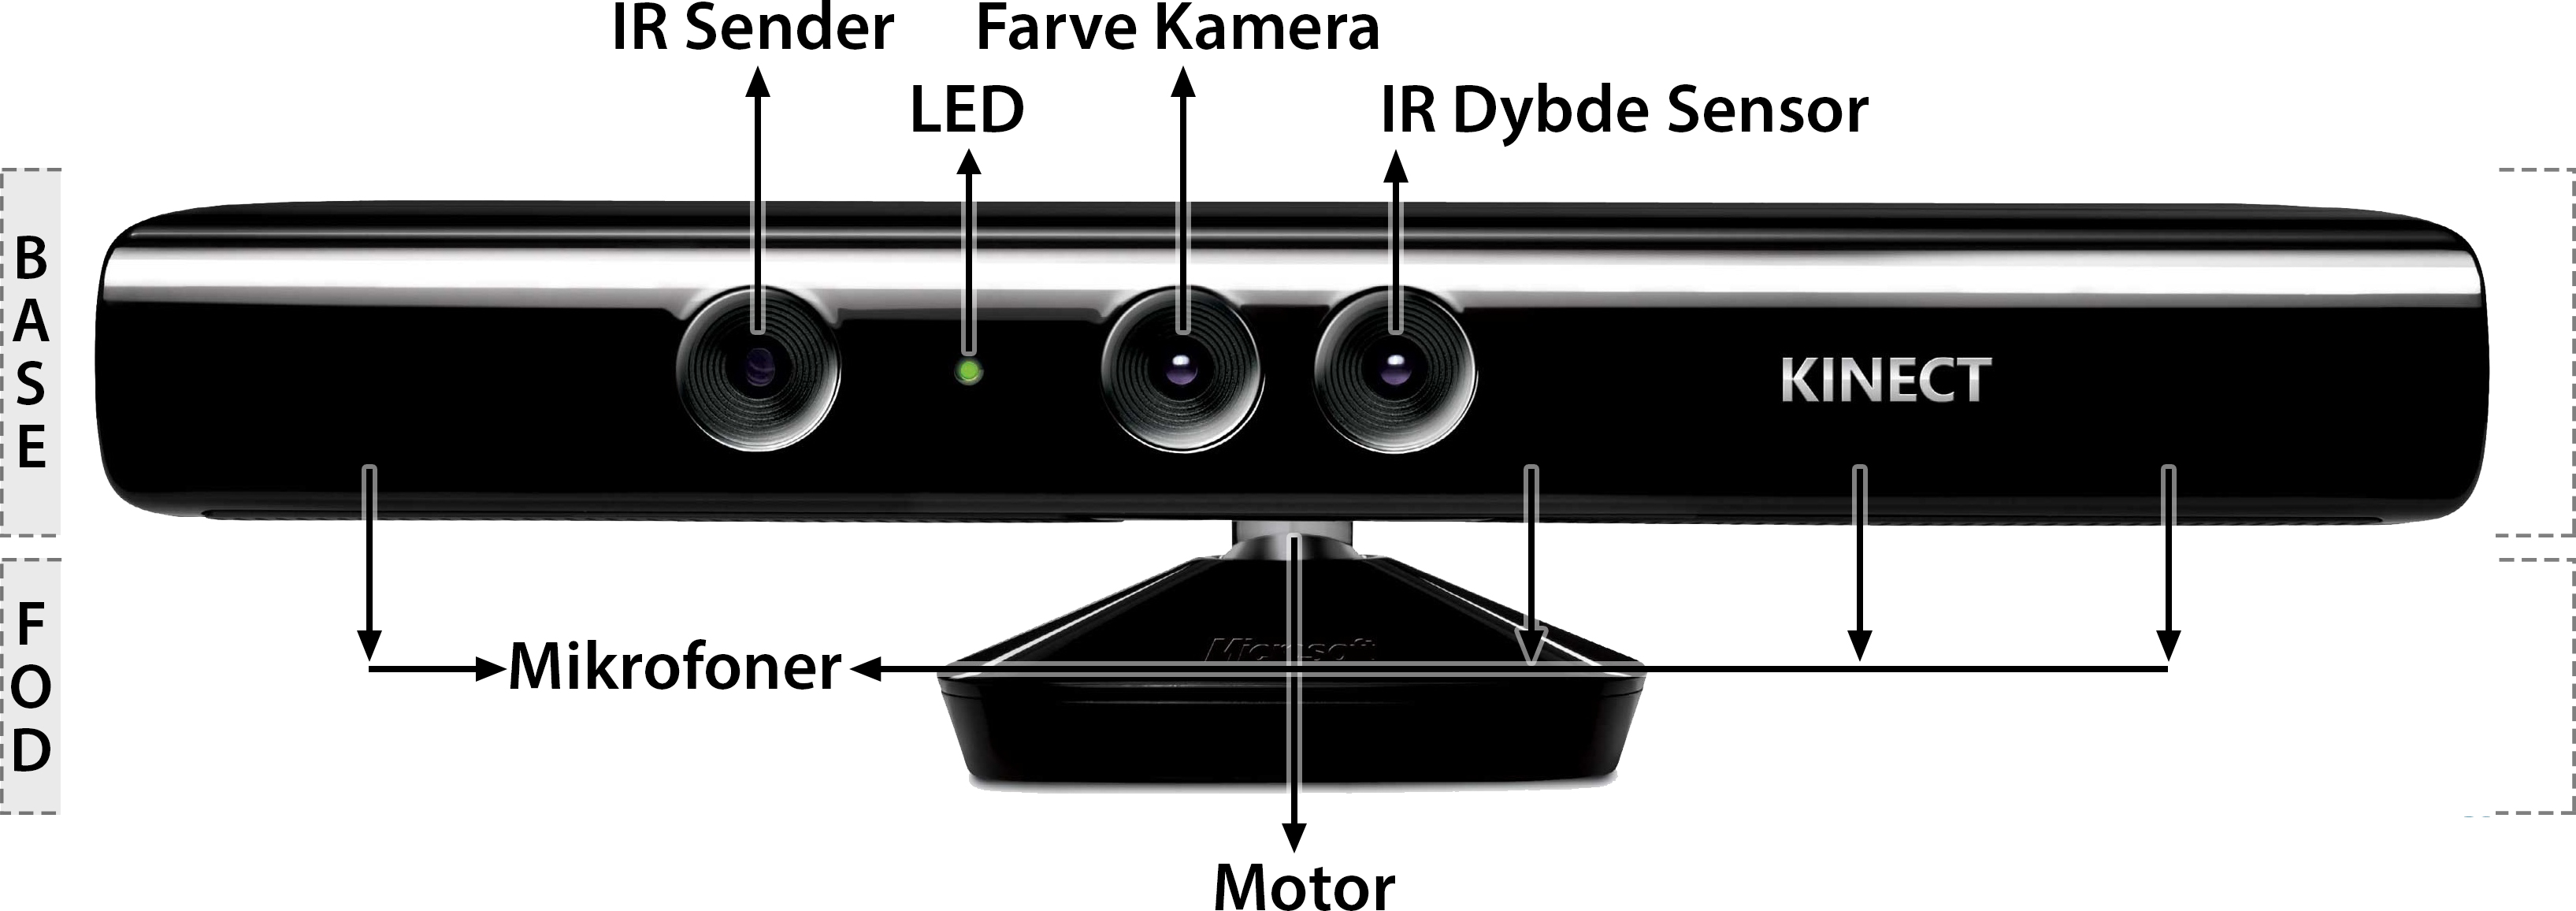
\includegraphics[width=\textwidth, clip, trim = 10cm 2cm 10cm 5cm]{./verden/kinect}
\caption{Kinecten monteret på en loftsplade.}
\label{testmiljo:kinect}
\end{figure}